\documentclass{article}

\usepackage{styles/arxiv}

\usepackage[utf8]{inputenc} % allow utf-8 input
\usepackage[T1]{fontenc}    % use 8-bit T1 fonts
\usepackage{hyperref}       % hyperlinks
\usepackage{url}            % simple URL typesetting
\usepackage{booktabs}       % professional-quality tables
\usepackage[english]{babel}
\usepackage{nicefrac}       % compact symbols for 1/2, etc.
\usepackage{microtype}      % microtypography
\usepackage{graphicx}
\usepackage{stmaryrd}

\usepackage{amsthm}
\usepackage{amssymb}
\usepackage{amsfonts}
\usepackage{amsmath}
\usepackage{mathtools}

\usepackage{tikz}
\usepackage{qtree}

\newtheorem{definition}{Definition}
\numberwithin{definition}{section}
\newtheorem{lemma}{Lemma}
\numberwithin{lemma}{section}
\newtheorem{proposition}{Proposition}
\numberwithin{proposition}{section}
\newtheorem{corollary}{Corollary}
\numberwithin{corollary}{section}
\newtheorem{theorem}{Theorem}
\numberwithin{theorem}{section}

\DeclareMathSymbol{\mathinvertedexclamationmark}{\mathclose}{operators}{'074}
\DeclareMathSymbol{\mathexclamationmark}{\mathclose}{operators}{'041}
\makeatletter
\newcommand{\raisedmathinvertedexclamationmark}{%
  \mathclose{\mathpalette\raised@mathinvertedexclamationmark\relax}%
}
\newcommand{\raised@mathinvertedexclamationmark}[2]{%
  \raisebox{\depth}{$\m@th#1\mathinvertedexclamationmark$}%
}
\begingroup\lccode`~=`! \lowercase{\endgroup
  \def~}{\@ifnextchar`{\raisedmathinvertedexclamationmark\@gobble}{\mathexclamationmark}}
\mathcode`!="8000
\makeatother

\newcommand{\intga}{\mathclap{\smash{\oplus}}{\int}}
\newcommand{\intgp}{\mathclap{\smash{\otimes}}{\int}}
\newcommand{\intgg}{\mathclap{\rightsquigarrow}\mathclap{\int}}

\title{Geometry of arithmetic expressions}

%\date{September 9, 1985}	% Here you can change the date presented in the paper title
%\date{} 					% Or removing it

\author{
  Mingli~Yuan \\
  AI Lab \\
  ColorfulClouds Tech.\\
  Beijing, 100083 \\
  \texttt{mingli.yuan@gmail.com}
  \And
  Le~Zhang \\
  %% Affiliation \\
  %% Address \\
  %% \texttt{email} \\
  \And
  Wenfeng~Jiang \\
  %% Affiliation \\
  %% Address \\
  %% \texttt{email} \\
}

% Uncomment to remove the date
%\date{}

% Uncomment to override  the `A preprint' in the header
\renewcommand{\headeright}{A preprint}
\renewcommand{\undertitle}{A preprint}

\begin{document}
\maketitle

\begin{abstract}
    TODO
\end{abstract}

\keywords{arithmetic expressions, hyperbolic geometry}

\setcounter{tocdepth}{2}
\tableofcontents
\newpage

\section{Introduction}\label{sec:introduction}

Can arithmetic expressions form a geometry space? What properties do these spaces hold? Can they apply to other domains
of mathematics? In this paper, we will show several examples and explore these topics step by step.

\subsection{An addition-multiplication grid}

For the upper half plane
\[
\{\mathcal{H}: (x, y) | y > 0 \}
\]

equipped with an inner product

\[
\mathbf{a} \cdot \mathbf{b} = \begin{bmatrix} a_x & a_y \end{bmatrix} \begin{bmatrix} \frac{1}{y^2} & 0 \\ 0 & \frac{1}{y^2} \end{bmatrix} \begin{bmatrix} b_x \\ b_y \end{bmatrix}
\]

and the metrics

\[
ds^2 = \frac{dx^2 + dy^2}{y^2}
\]

We have the Gauss curvature of $-1$ and the Laplacian is

\[
\Delta = - y^2 (\frac{\partial^2}{\partial x^2} + \frac{\partial^2}{\partial y^2})
\]

We consider a scalar field satisfying

\begin{equation}
A = - \frac{x}{y}
\end{equation}

\begin{figure}[ht]
\centering
\resizebox{0.9\textwidth}{!}{\includegraphics{images/01-grid-example-1.pdf}}
\caption{An addition-multiplication grid by generators with $\mu=1$ and $\lambda=\ln2$}\label{fig:gridex0}
\end{figure}

Now we can draw a grid on $\mathcal{H}$. In the above figure \ref{fig:gridex0},
the blue lines encode $+ 1$ relationship, the green lines encode $\times 2$ relationship,
and they are line families that are perpendicular each other.
The length of the line segments between two neighbor crossing point are unit length.
The red value of the crossing point is the value of the scalar field $A$ at that point.
Considering the relationships the lines encoded, we can then encode threadlike arithmetic expressions
which will be introduced in next subsection.

The addition-multiplication grid is also scale invariant.

\subsection{Threadlike arithmetic expressions}

Given any arithmetic expression, such as

$$
(1 \times 2 \times 2 - 1) \times (2 + 1) - 6
$$

we can parse them into a syntax trees. For example, the above expression can be parsed into

\begin{figure}[ht]
\centering
\resizebox{0.2\textheight}{!}{\includegraphics{images/02-example-expression-syntax-tree.pdf}}
\caption{a syntax tree of which is not threadlike}\label{fig:syntaxtree}
\end{figure}

The evaluation of the expression is from the leaves to the root recursively, but generally the orders of such evaluations are not unique.
For one expression, if the sequence of evaluations is unique, we call it a threadlike expression.

\begin{definition}
A threadlike expression is an arithmetic expression with a unique evaluation sequence.
\end{definition}

It is obvious that there are two kind of threadlike expressions, left-expanded and right-expanded, such as

\begin{figure}[ht]
\centering
\resizebox{0.4\textheight}{!}{\includegraphics{images/03-example-expression-syntax-tree-left-right.pdf}}
\caption{two kind of threadlike expressions, left-expanded and right-expanded}\label{fig:leftright}
\end{figure}


\subsection{Encoding of threadlike expressions}


\section{Flow equation and the first kind of arithmetic expression space}\label{sec:examples}

\subsection{Flow equation}

Considering an infinitesimal generation process over a Riemannian surface $M$ with one generator for additional action $\mu$
and the other for multiplicative action $e^\lambda$, the two generators are perpendicular. And then,
under this generation process, we get an assignment $A: M \to R$ over the surface.

At any point with an assigment $a_0$, considering a moving with distance of $\epsilon$, direction angle of $\theta$,
time elapse of $\delta$, we can establish

\begin{equation}
    a_{\delta} = (a_0 + \mu \epsilon \cos \theta)e^{\lambda \epsilon \sin \theta}
\end{equation}

or

\begin{equation}
    a_{\delta} = a_0 e^{\lambda \epsilon \sin \theta} + \mu \epsilon \cos \theta
\end{equation}

Both can be simplified to the same

\begin{equation}
    a_{\delta} = a_0 + \epsilon (a_0 \lambda \sin \theta + \mu \cos \theta)
\end{equation}

Then

\begin{equation}
    \frac{1}{\delta} (a_{\delta} - a_0) = \frac{\epsilon}{\delta} (\mu \cos \theta + x_0 \lambda \sin \theta)
\end{equation}

When both $\delta$ and $\epsilon$ are towards zero, we get $da / dt$, and hence

\begin{equation}
    \frac{da}{dt} = u (\mu \cos \theta + a \lambda \sin \theta)
\end{equation}

Or, we can change it to other forms

\begin{equation}
    \frac{da}{ds} = \mu \cos \theta + a \lambda \sin \theta\label{eq:flow}
\end{equation}

The left side of flow equation\eqref{eq:flow} is governed by the distance structure, and the right side is governed by the angle structure,
and these lead to a theorem.

\begin{theorem}
Isometries keep the flow equation\eqref{eq:flow}
\label{thm:isometry}
\end{theorem}

\subsection{Example I}\label{subsec:exmp1}

\begin{theorem}\footnote{The proof is originally by Le Zhang, and modified by Mingli Yuan}
For the above $A$, $A$ satisfy the flow equation\eqref{eq:flow}
\end{theorem}

\begin{proof}
$$
da = d(-\frac{x}{y}) = \frac{xdy - ydx}{y^2} = -\frac{dx + ady}{y}
$$

and

$$
ds = \frac{\sqrt{dx^2 + dy^2}}{y}
$$

then

$$
\frac{da}{ds} = - \frac{dx + ady}{y} \frac{y}{\sqrt{dx^2 + dy^2}} = - \frac{dx + ady}{\sqrt{dx^2 + dy^2}}
$$

Considering the local coordinate is given by $(-1, 0)$ 和 $(0, -1)$ under the right-hand rule, we have

$$
\cos \theta = \frac{\begin{bmatrix} dx & dy \end{bmatrix} \begin{bmatrix} \frac{1}{y^2} & 0 \\ 0 & \frac{1}{y^2} \end{bmatrix} \begin{bmatrix} -1 \\ 0 \end{bmatrix}}{\sqrt{\begin{bmatrix} dx & dy \end{bmatrix} \begin{bmatrix} \frac{1}{y^2} & 0 \\ 0 & \frac{1}{y^2} \end{bmatrix} \begin{bmatrix} dx \\ dy \end{bmatrix}}\sqrt{\begin{bmatrix} -1 & 0 \end{bmatrix} \begin{bmatrix} \frac{1}{y^2} & 0 \\ 0 & \frac{1}{y^2} \end{bmatrix} \begin{bmatrix} -1 \\ 0 \end{bmatrix}}}
$$

hence

$$
\cos \theta = \frac{-dx}{\sqrt{dx^2 + dy^2}}
$$

and similarly

$$
\sin \theta = \frac{-dy}{\sqrt{dx^2 + dy^2}}
$$

then

$$
\frac{da}{ds} = \cos \theta + a \sin \theta
$$

\end{proof}

\subsubsection{As eigenvalue of Laplacian}

We can verify $A$ is an eigenvalue of the Laplacian

$$
\Delta A = - y^2 (\frac{\partial^2}{\partial x^2} A + \frac{\partial^2}{\partial y^2} A) = y^2 (\frac{1}{\partial y} (\frac{1}{\partial y} \frac{x}{y})) = 2 A
$$

\subsection{Example II}\label{subsec:exmp2}

\subsubsection{Geometry settings}\label{subsec:gsetting2}

First, we introduce the horocycle-based coordinate system of hyperbolic surfaces.
It is a global coordinate system given by two orthogonal pencils of circles; one pencil are horocycles sharing the same ideal point,
the other are geodesics which are perpendicular to the first pencil.

On the Poincaré disc $\mathcal{P}$, the blue horocycles are tangible each other at the ideal point $\Omega$, which forms the first pencil,
the green lines are geodesics forms the second pencil; and the coordinate of point $P$ are given by the length of $OQ$ and $QP$,
where the point $O$ is the origin and the length is the metric inside the hyperbolic surface.

The coordinate of $P$ is $(u,v)$ where the sign of the length is decided by below rules:
\begin{itemize}
    \item u: if $P$ is in the same side of $\Omega$, then x is positive; otherwise x is negative
    \item v: the sign of the length should satisfy the right-hand rule
\end{itemize}

\begin{figure}[ht]
\centering
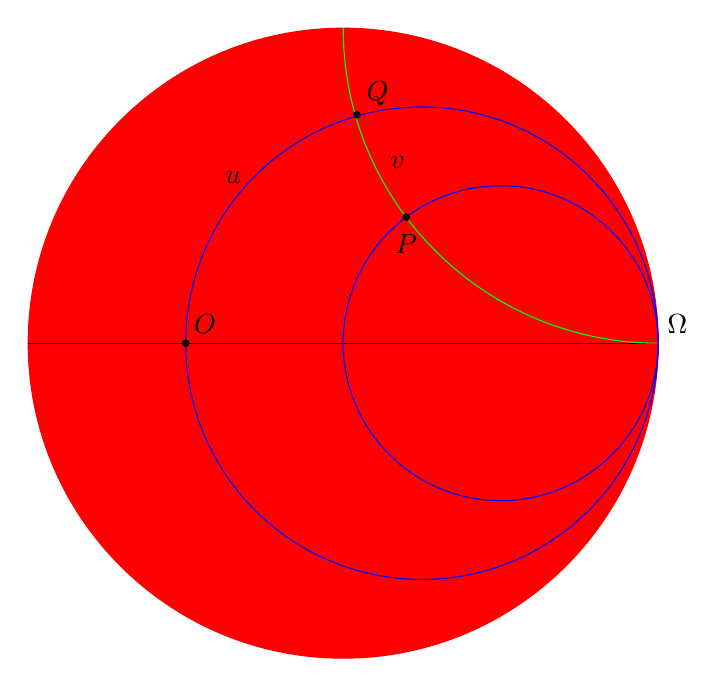
\begin{tikzpicture}
    \node[anchor=225] at (4,2) {$\Omega$};
    \draw[red,fill=red] (0,2) circle[radius=4];
    \draw[blue] (1, 2) circle[radius=3];
    \draw[black] (-4,2) -- (4,2);
    \draw[green] (4,2) arc (-90:-180:4);
    \draw[blue] (2, 2) circle[radius=2];
    \node[fill,circle,inner sep=1pt] at (-2,2) {};
    \node[anchor=225] at (-2,2) {$O$};
    \node[fill,circle,inner sep=1pt] at (0.175,4.9) {};
    \node[anchor=225] at (0.175,4.9) {$Q$};
    \node[fill,circle,inner sep=1pt] at (0.8,3.6) {};
    \node[anchor=90] at (0.8,3.5) {$P$};
    \node[anchor=225] at (0.49,4.1) {$v$};
    \node[anchor=225] at (-1.6,3.9) {$u$};
\end{tikzpicture}
\caption{Horocycle-based coordinate system}\label{fig:horocyclecoord}
\end{figure}

We can equip it with an inner product

\[
\mathbf{a} \cdot \mathbf{b} = \begin{bmatrix} a_u & a_v \end{bmatrix} \begin{bmatrix} e^{-2v} & 0 \\ 0 & 1 \end{bmatrix} \begin{bmatrix} b_u \\ b_v \end{bmatrix}
\]

and the metrics

$$
ds^2 = e^{-2v} du^2 + dv^2
$$

\subsubsection{The assignment}

\begin{equation}
A = u e^{-v}
\end{equation}

\begin{theorem}
For the above $A$, $A$ satisfy the flow equation\eqref{eq:flow}
\end{theorem}

\begin{figure}[ht]
\centering
\begin{tikzpicture}
\draw [black, line width=0.6pt, ->] (0,0) to[out=90,in=270] (0,4.25);
\node [anchor=south] at (0,4.5) {y};
\draw [black, line width=0.6pt, ->] (-4.25,0) to[out=0,in=180] (4.25,0);
\node [anchor=west] at (4.5,0) {x};

\draw [blue, line width=0.6pt] (-4.25,4.0) to[out=0,in=180] (4.25,4.0);
\draw [blue, line width=0.6pt] (-4.25,2.0) to[out=0,in=180] (4.25,2.0);
\draw [green, line width=0.6pt] (-3.5,0) to[out=90,in=270] (-3.5,4.5);

\node[anchor=45] at (0.0,4.0) {$O$};
\node[anchor=45] at (-3.5,4.0) {$Q$};
\node[anchor=45] at (-3.5,2.0) {$P$};
\node[anchor=225] at (-2.0,4.1) {$x = u$};
\node[anchor=225] at (-3.0,1.0) {$y = e^v$};

\end{tikzpicture}

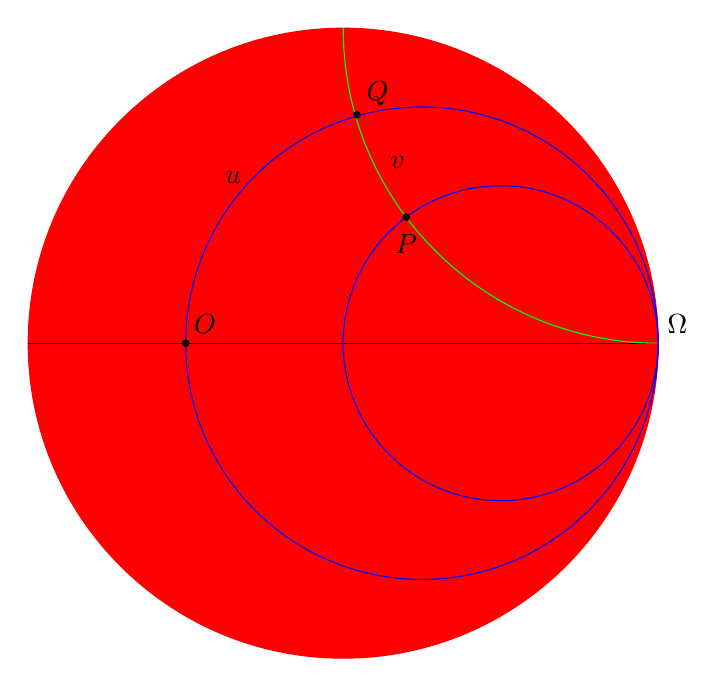
\begin{tikzpicture}
    \node[anchor=225] at (4,2) {$\Omega$};
    \draw[red,fill=red] (0,2) circle[radius=4];
    \draw[blue] (1, 2) circle[radius=3];
    \draw[black] (-4,2) -- (4,2);
    \draw[green] (4,2) arc (-90:-180:4);
    \draw[blue] (2, 2) circle[radius=2];
    \node[fill,circle,inner sep=1pt] at (-2,2) {};
    \node[anchor=225] at (-2,2) {$O$};
    \node[fill,circle,inner sep=1pt] at (0.175,4.9) {};
    \node[anchor=225] at (0.175,4.9) {$Q$};
    \node[fill,circle,inner sep=1pt] at (0.8,3.6) {};
    \node[anchor=90] at (0.8,3.5) {$P$};
    \node[anchor=225] at (0.49,4.1) {$v$};
    \node[anchor=225] at (-1.6,3.9) {$u$};
\end{tikzpicture}
\caption{Mapping between two examples}\label{fig:mapping}
\end{figure}

\begin{proof}

For example in last section \ref{subsec:exmp1}, if we introduce complex

$$
z = x + y i
$$

and there is a Möbius transform

$$
z \mapsto \frac{z-i}{z+i}
$$

that can connect the upper half plane model in last section \ref{subsec:exmp1} to current Horocycle-based coordinate system.

This transform maps each horizontal lines in $\mathcal{H}$ into the horocycles sharing the same ideal point $\Omega = 1$ in $\mathcal{P}$,
also it maps each vertical geodesics in $\mathcal{H}$ into geodesics in $\mathcal{P}$ which are perpendicular to the above horocycles.

And rewrite the Möbius transform in the target coordinate, we get:

$$
\begin{cases}
x = u\\
y = e^v \\
\end{cases}
$$

This lead to

$$
A = -\frac{x}{y} = u e^{-v}
$$

And because of theorem \ref{thm:isometry} and Möbius transform is conformal, we can conclude that $A = u e^{-v}$ obey flow equation.

\end{proof}

\subsubsection{As eigenvalue of Laplacian}

Laplacian is given by\cite{Costa2001ADO}

$$
\Delta = e^{2y} \frac{\partial^2}{{\partial x}^2} + \frac{\partial^2}{{\partial y}^2} - \frac{\partial}{\partial y}
$$

and we have $A$ is an eigenvalue of the Laplacian
$$
\Delta A = e^{2y} \frac{\partial^2(x e^{-y})}{{\partial x}^2} + \frac{\partial^2(x e^{-y})}{{\partial y}^2} - \frac{\partial(x e^{-y})}{\partial y} = 2A
$$

\section{Arithmetic expression, LISP and transformation over trees}\label{sec:expressions}


\subsection{Donaghey transformation}\label{sec:donaghey}



\begin{thebibliography}{9}

\bibitem{Giuseppe2019}
    Giuseppe Negro,
    \textit{Laplacian on Poincaré upper half plane},
    Mathematics Stack Exchange,
    2019.

\bibitem{Costa2001ADO}
  S. Costa,
  \textit{A description of several coordinate systems for hyperbolic spaces},
  arXiv: Mathematical Physics,
  2001.


\end{thebibliography}


\end{document}
